
%!TEX program = xelatex
\documentclass[letterpaper,12pt]{exam}
\usepackage{../videoNotes}
\usepackage{xcolor}
\usepackage[dvipsnames]{xcolor}
\usepackage{soul}
\newcommand{\unit}{Unit 06}

\usepackage{draftwatermark}
\SetWatermarkText{DRAFT}
\SetWatermarkScale{1.5}
\SetWatermarkColor{red!20}

\pagestyle{headandfoot}
\firstpageheader{CSC 264 \semester\ \  \unit}{}{Name: $\rule{6cm}{0.15mm}$}
\runningheader{CSC 264 \semester}{\unit}{Page \thepage\ of \numpages}
\firstpagefooter{}{}{}
\runningfooter{}{}{}

\begin{document}

%\underconstruction

\section*{\unit\_005 -- Syntax}
\par{\fontfamily{qzc}\selectfont\textbf{Video Length 12:45}}
\begin{questions}

\begin{samepage}
    \question What is the difference between .ascii and the .asciz directive?
    \vspace{5mm}
\end{samepage}
\begin{samepage}
    \question How many bytes would the command \textbf{\texttt{.ascii "dog"}} allocate?
    \vspace{5mm}
\end{samepage}
\begin{samepage}
    \question How many bytes would the command \textbf{\texttt{.asciz "dog"}} allocate?
    \vspace{5mm}
\end{samepage}
\par
\begin{samepage}
    \question The code below declares a string.  Write the declaration of \texttt{len} that has the assembler calculate the lenght of word.
    \begin{verbatim}
         message: .ascii "Hello, World!"
         len:     .quad   
    \end{verbatim}        
    \vspace{5mm}
\end{samepage}
\par
 \begin{samepage}
     \question Modify the code below to load the address of message into the rdi register.
        \begin{verbatim}
            movq  letters, %rdi
        \end{verbatim}
     \vspace{5mm}
 \end{samepage}
 \par
 \begin{samepage}
     \question Modify the code below to load the contents of rdi into the r8b register.
        \begin{verbatim}
            movb  %rdi , %r8b
        \end{verbatim}
     \vspace{5mm}
 \end{samepage}
 \par 
 \question Consider the previous two questions.  One of them was moving a quad.  The second was only moving a byte.  Explain why.
\vspace{5mm}
 %----------------------------------

\section*{\unit\_010 -- Syscall}
\par{\fontfamily{qzc}\selectfont\textbf{Video Length 11:30}}
\begin{samepage}
    \question What is syscall?  Why do we need it?
    \vspace{5mm}
\end{samepage}
\par
\begin{samepage}
    \question Suppose you wanted to convert a program written for x86-64 to run on an ARM processor.  Would syscall need to be adapted to run on ARM?
    \vspace{5mm}
\end{samepage}
\par
 \begin{samepage}
     \question What three registers will we be using to communicate with syscall?
     \vspace{5mm}
 \end{samepage}
 \par
 \begin{samepage}
     \question If syscall is considered a function call, how are parameters passed to the function?
     \vspace{5mm}
 \end{samepage}
 \par
   
\rule{0.5\textwidth}{.4pt} %End of section
%----------------------------------



\end{questions} 
%footer
\begin{center}
    \rule{0.667\textwidth}{.8pt} %End of section
\end{center}


If you have any lingering questions or problems, please write them here or see me.
\vfill
\begin{center}
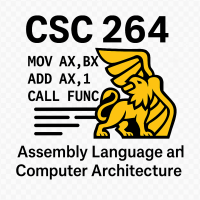
\includegraphics{../csc264Logo}
\end{center}
\end{document} 